% ============================================================
%  SEKCJA: Analiza stabilności centroidu naukowca
%  Wklej do dokumentu głównego; wykresy umieść w katalogu figures/
%  Wymagane pakiety: graphicx, booktabs, float, amsmath, caption, subcaption
% ============================================================

\section{Analiza stabilności centroidu profilu naukowca}
\label{sec:centroid-stability}

% ----------------------------------------------------------
\subsection{Motywacja}
% ----------------------------------------------------------

Profil embeddingowy naukowca wyznaczamy jako \emph{centroid} -- średnią wektorów
reprezentujących poszczególne publikacje:
\begin{equation}
    \mathbf{c}_S \;=\; \frac{1}{|S|} \sum_{i \in S} \mathbf{e}_i,
    \label{eq:centroid}
\end{equation}
gdzie $\mathbf{e}_i \in \mathbb{R}^d$ jest embeddingiem $i$-tej pracy
i~$S$ -- wybranym podzbiorem prac naukowca.
Kluczowym pytaniem praktycznym jest: \textbf{ile publikacji potrzeba,
by centroid $\mathbf{c}_S$ był wiarygodną aproksymacją centroidu
pełnego $\mathbf{c}_\text{all}$, wyznaczonego ze wszystkich dostępnych prac?}
Odpowiedź ma bezpośrednie znaczenie dla jakości systemu rekomendacji --
naukowcy z~małym dorobkiem nie powinni być z~góry dyskwalifikowani,
jeśli już kilka prac wystarcza do uformowania stabilnego profilu.

% ----------------------------------------------------------
\subsection{Dane i metodologia}
% ----------------------------------------------------------

\subsubsection{Zbiór danych i modele embeddingowe}

Eksperymenty przeprowadzono na zbiorze $N = 164$ pracowników naukowych
Uniwersytetu im.~Adama Mickiewicza w~Poznaniu.
Dla każdej ze~$3\,440$ zidentyfikowanych publikacji wyznaczono embedding
\emph{tytułu} przy użyciu sześciu modeli transformerowych (Tabela~\ref{tab:models}).

\begin{table}[H]
\centering
\caption{Modele embeddingowe użyte w~eksperymencie.}
\label{tab:models}
\begin{tabular}{llcc}
\toprule
\textbf{Skrót} & \textbf{Identyfikator modelu} & \textbf{Wymiar} & \textbf{Domena} \\
\midrule
MiniLM-L6          & \texttt{all-MiniLM-L6-v2}                          & 384 & ogólny \\
Specter             & \texttt{allenai/specter}                             & 768 & naukowy \\
MPNet-Base          & \texttt{all-mpnet-base-v2}                          & 768 & ogólny \\
Multilingual-MiniLM & \texttt{paraphrase-multilingual-MiniLM-L12-v2}     & 384 & wielojęz. \\
MiniLM-L12          & \texttt{all-MiniLM-L12-v2}                         & 384 & ogólny \\
BGE-Small           & \texttt{BAAI/bge-small-en-v1.5}                    & 384 & retrieval \\
\bottomrule
\end{tabular}
\end{table}

Modele o~wymiarze $768$ (Specter, MPNet-Base) sprowadzono do wymiaru $384$
za~pomocą \emph{losowej projekcji liniowej} opartej na~lemacie
Johnsona--Lindenstraussa~\cite{johnson1984extensions}.
Dla wektora $\mathbf{e} \in \mathbb{R}^{768}$ projekcja przyjmuje postać:
\begin{equation}
    \mathbf{e}' \;=\; \frac{1}{\sqrt{384}}\,\mathbf{e}\,\mathbf{P},
    \qquad \mathbf{P} \in \mathbb{R}^{768 \times 384},\; P_{ij} \sim \mathcal{N}(0,1),
    \label{eq:jl}
\end{equation}
po~czym $\mathbf{e}'$ normalizowano do~normy jednostkowej~$L_2$.
Macierz $\mathbf{P}$ jest deterministyczna (ustalono ziarno losowości),
dzięki czemu wyniki są w~pełni powtarzalne.
Liniowość projekcji gwarantuje, że
$\operatorname{resize}(\bar{\mathbf{e}}) = \overline{\operatorname{resize}(\mathbf{e})}$,
tzn.\ centroid z~przeskalowanych wektorów jest równoważny przeskalowaniu
gotowego centroidu.

\subsubsection{Miara stabilności}

Jako miarę zbieżności centroidu podzbioru do centroidu pełnego stosujemy
\textbf{podobieństwo cosinusowe}:
\begin{equation}
    \mathrm{sim}(\mathbf{c}_S,\,\mathbf{c}_\text{all})
    \;=\;
    \frac{\mathbf{c}_S \cdot \mathbf{c}_\text{all}}
         {\|\mathbf{c}_S\|\;\|\mathbf{c}_\text{all}\|}.
    \label{eq:cosine}
\end{equation}
Wartość~1 oznacza identyczny kierunek w~przestrzeni wektorowej
(profil zbudowany z~podzbioru jest identyczny z~profilem pełnym);
wartości bliskie~0 wskazują na~brak korelacji między centroidami.
Za progi praktycznej stosowalności przyjęto $\mathrm{sim} \geq 0{,}95$
(dopuszczalne odchylenie) oraz $\mathrm{sim} \geq 0{,}99$ (wysoka wierność).

\subsubsection{Schemat eksperymentu}

Przeprowadzono trzy eksperymenty:

\begin{enumerate}
    \item \textbf{Eksperyment pilotażowy (Exp1).}
    Jeden naukowiec -- prof.~UAM dr~hab.~Tomasz~Górecki
    (ORCID: \texttt{0000-0002-9969-5257}, $n_\text{all} = 114$ prac) --
    jako reprezentatywny przypadek naukowca o~szerokim i~interdyscyplinarnym dorobku
    (statystyka funkcjonalna, klasyfikacja szeregów czasowych, chemometria).
    Dla rozmiarów próbki $k \in \{3, 5, 10\}$ wygenerowano po~3 losowe podzbiory;
    dodatkowo wyznaczono centroid ze~wszystkich 114~prac.

    \item \textbf{Eksperyment rozszerzony -- gęste próbkowanie (Exp2).}
    Dla tego samego naukowca wygenerowano po~$K = 300$ unikalnych losowych
    podzbiorów dla każdego rozmiaru $k \in \{3, 5, 10, 20, 30, 50, 100\}$
    (rozmiar~$k=150$ pominięto, ponieważ naukowiec ma jedynie 114~prac).
    Łącznie $300 \times 7 + 1 = 2\,101$ centroidów na~model.
    Unikalne podzbiory gwarantowano przez śledzenie zbioru wygenerowanych
    zestawów (struktura \texttt{frozenset}); powtórzenia między różnymi
    rozmiarami~$k$ były dozwolone.

    \item \textbf{Eksperyment zbiorczy -- 107~naukowców (Exp3).}
    Eksperyment rozszerzono na~wszystkich 107~naukowców UAM posiadających
    co~najmniej 3~prace w~zbiorze danych (mediana: 20~prac, max: 199~prac).
    Dla każdego naukowca, modelu i~rozmiaru $k \in \{3, 5, 10, 20, 50, 100\}$
    wygenerowano po~$N = 10$ losowych podzbiorów.
    Wyniki uśredniono po~naukowcach.
\end{enumerate}

% ----------------------------------------------------------
\subsection{Wyniki}
% ----------------------------------------------------------

\subsubsection{Eksperyment pilotażowy -- wizualizacja PCA}

Rysunek~\ref{fig:pca_centroid} przedstawia centroidy prof.~Góreckiego
zrzutowane na~płaszczyznę dwóch głównych składowych (PCA na~znormalizowanych
$L_2$ wektorach centroidów).
Każdy punkt odpowiada centroidowi zbudowanemu z~$k \in \{3, 5, 10\}$~losowych prac;
gwiazdka oznacza centroid pełny (wszystkie 114~prac).

\begin{figure}[H]
    \centering
    
\includegraphics[width=\textwidth]{pubs_num_stability/pca_centroid_stability.png}
    \caption{Wizualizacja PCA centroidów prof.~UAM dr~hab.~Tomasza Góreckiego
    dla sześciu modeli embeddingowych (3~powtórzenia na~rozmiar próbki).
    Czerwone punkty ($k=3$), żółte ($k=5$), niebieskie ($k=10$),
    zielona gwiazdka -- centroid ze~wszystkich 114~prac.
    Skupienie punktów wokół gwiazdki oznacza wysoką stabilność centroidu.}
    \label{fig:pca_centroid}
\end{figure}

Widoczna jest wyraźna różnica między modelami.
Dla \textbf{Spectera} i~\textbf{BGE-Small} wszystkie 9~centroidów
(niezależnie od~$k$) skupia się ściśle wokół centroidu pełnego --
nawet przy zaledwie 3~pracach centroid jest zbliżony do reprezentacji
opartej na~całym dorobku.
Dla modeli ogólnych (MiniLM-L6, MiniLM-L12, MPNet-Base,
Multilingual-MiniLM) centroidy przy $k=3$ są rozrzucone daleko
od~centroidu pełnego, a~dopiero przy $k=10$ zaczynają się skupiać.

\subsubsection{Macierze podobieństwa cosinusowego -- eksperyment pilotażowy}

\begin{figure}[H]
    \centering
    
\includegraphics[width=\textwidth]{pubs_num_stability/cosine_similarity_stability.png}
    \caption{Macierze podobieństwa cosinusowego między centroidami
    prof.~Góreckiego (eksperyment pilotażowy, 3~powtórzenia).
    Skala barw: czerwony~$\approx 0{,}7$ -- zielony~$\approx 1{,}0$.
    Etykiety osi: kolor czerwony~-- $k=3$, pomarańczowy~-- $k=5$,
    niebieski~-- $k=10$, zielony~-- centroid pełny (\textit{all}).}
    \label{fig:heatmap_basic}
\end{figure}

Rysunek~\ref{fig:heatmap_basic} potwierdza obserwację z~PCA.
W~przypadku \textbf{Spectera} i~\textbf{BGE-Small}
niemal cała macierz jest zielona -- nawet centroidy z~zaledwie 3~prac
wykazują podobieństwo $> 0{,}90$ do centroidu pełnego i~do siebie nawzajem.
W~przypadku modeli ogólnych komórki odpowiadające centroidom z~$k=3$
są wyraźnie czerwone ($\mathrm{sim} \approx 0{,}50$--$0{,}65$),
co~wskazuje na~dużą losowość profilu zbudowanego z~małej próbki prac.

\subsubsection{Eksperyment rozszerzony -- gęste próbkowanie}

\begin{figure}[H]
    \centering
    
\includegraphics[width=\textwidth]{pubs_num_stability/pca_dense_stability.png}
    \caption{Chmury 2\,101~centroidów prof.~Góreckiego w~przestrzeni PCA
    (eksperyment gęstego próbkowania, 300~losowych podzbiorów na~rozmiar).
    Gradient barw od~żółtego ($k=3$) przez fioletowy ($k=30$) do~jasno\-niebieskiego
    ($k=100$); gwiazdka~-- centroid pełny.
    Ścieśnienie chmury wraz ze~wzrostem $k$ świadczy o~rosnącej stabilności profilu.}
    \label{fig:pca_dense}
\end{figure}

\begin{figure}[H]
    \centering
    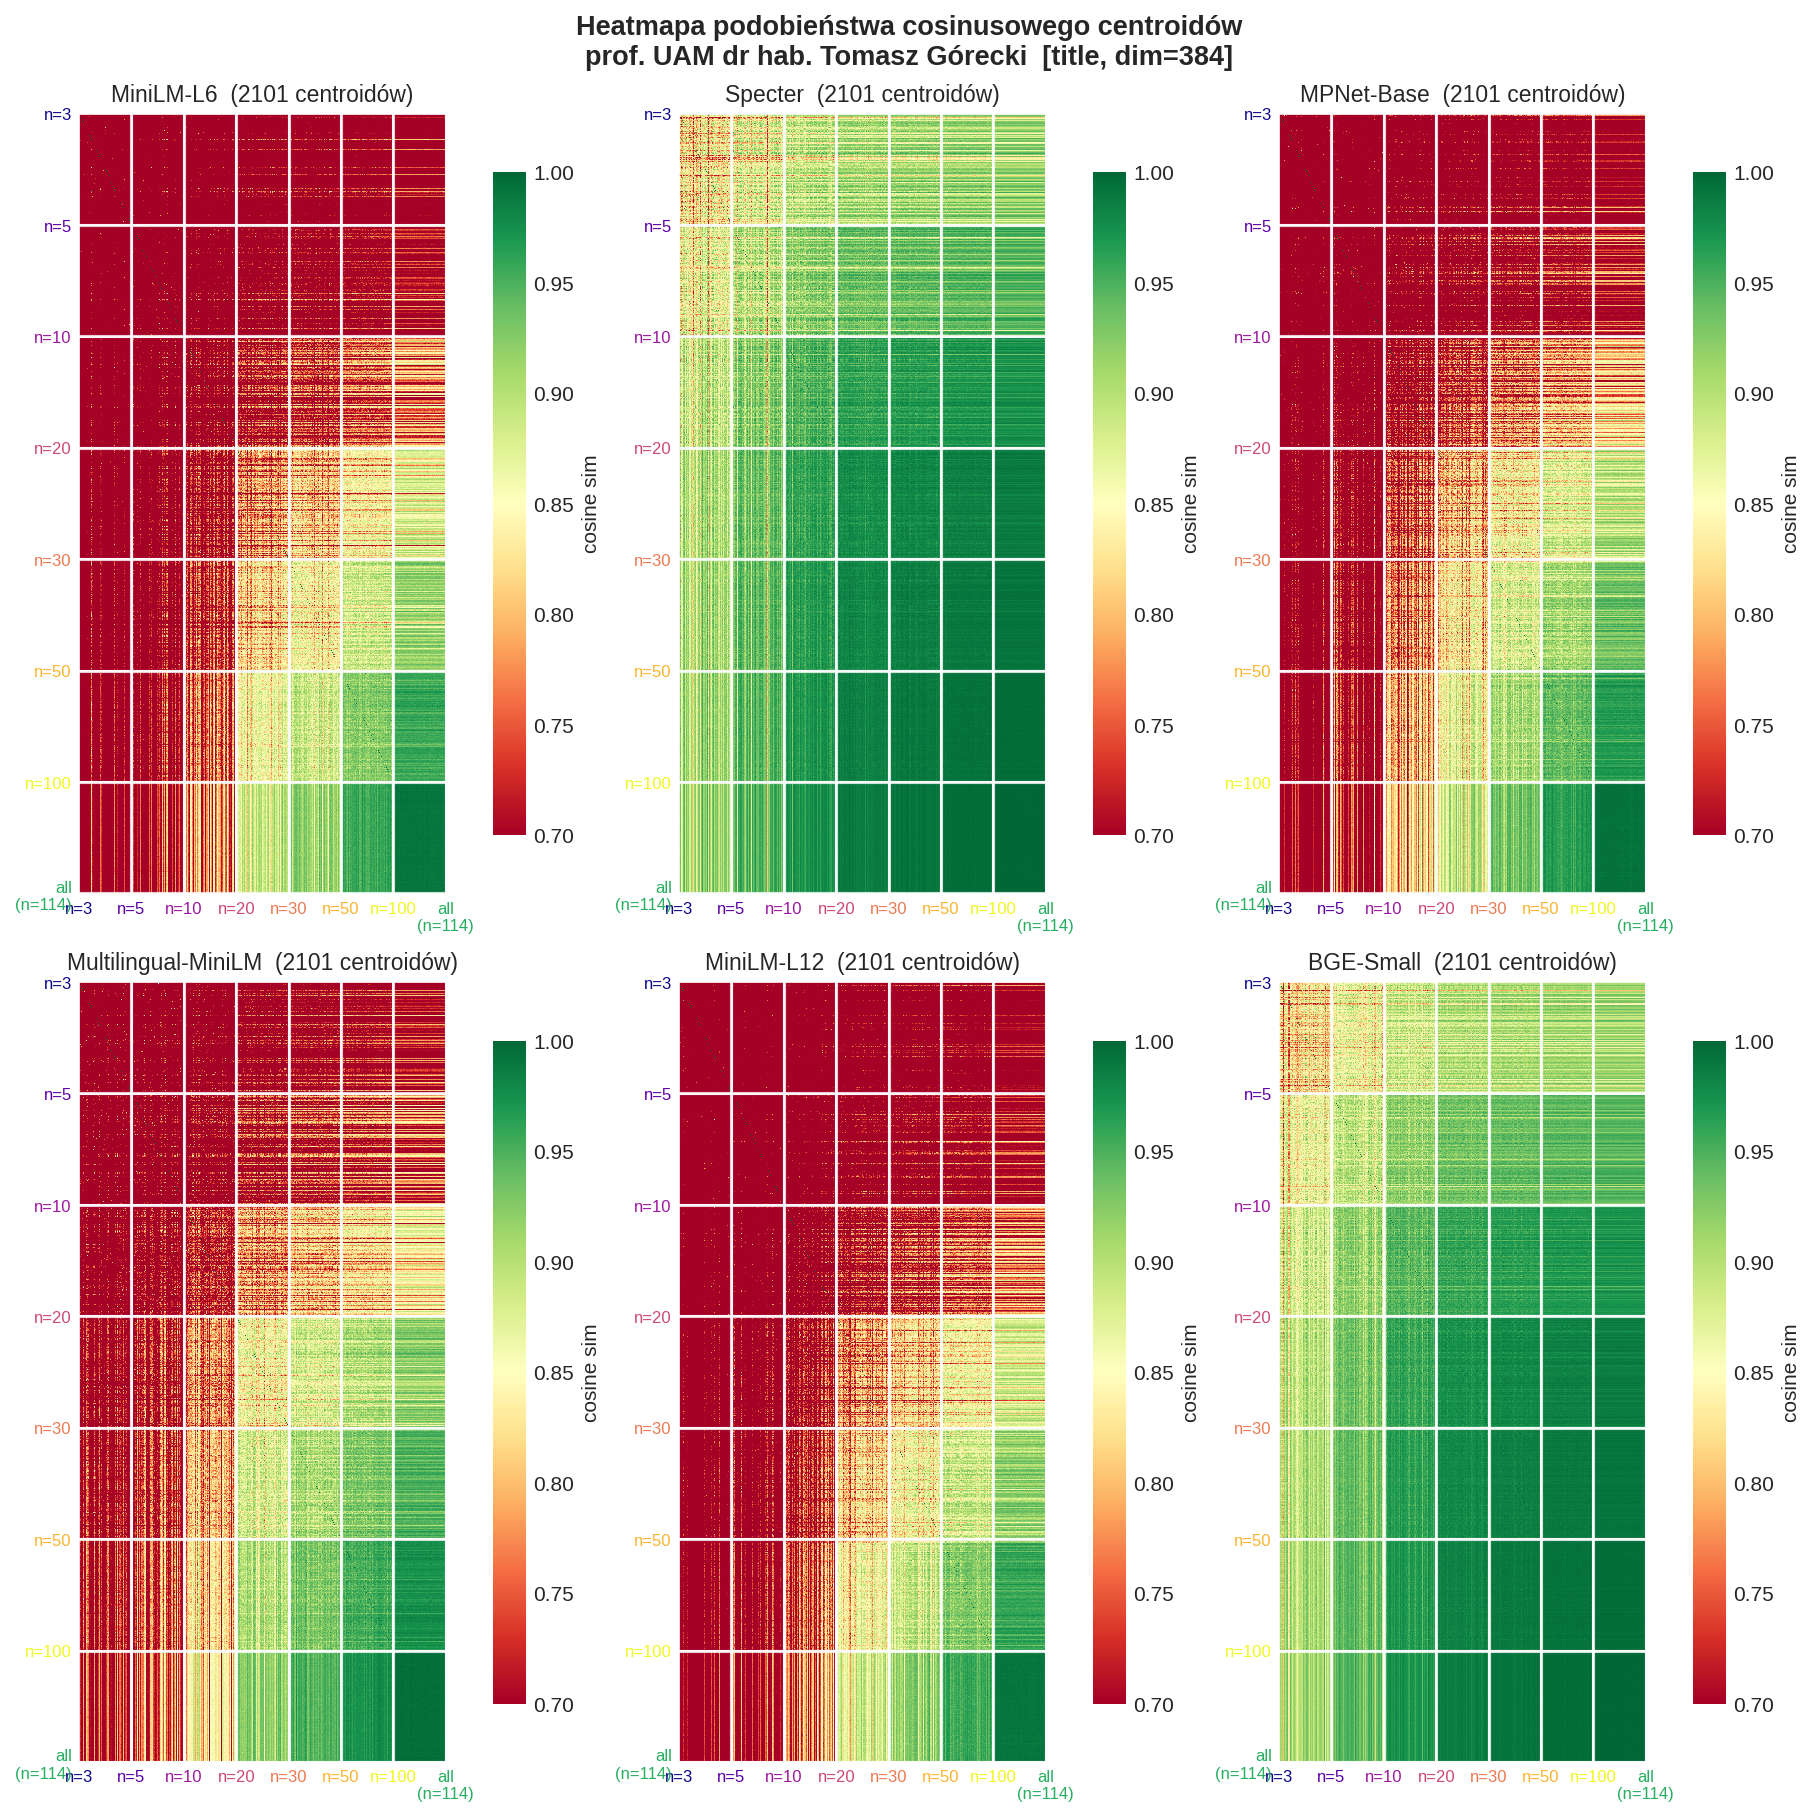
\includegraphics[width=\textwidth]{pubs_num_stability/heatmap_dense_stability.png}
    \caption{Heatmapa podobieństwa cosinusowego 2\,101~centroidów prof.~Góreckiego
    (eksperyment gęstego próbkowania).
    Oś posortowana wg rosnącego $k$; białe linie oddzielają grupy.
    Zielone bloki na~przekątnej dla Spectera i~BGE-Small wskazują,
    że~centroidy w~obrębie jednej grupy są do siebie bardzo podobne
    nawet przy małym~$k$.}
    \label{fig:heatmap_dense}
\end{figure}

Rysunek~\ref{fig:pca_dense} uwidacznia wyraźnie wzorzec konwergencji:
dla \textbf{Spectera} i~\textbf{BGE-Small} chmury wszystkich rozmiarów
są skupione blisko centroidu pełnego, a~różnica między $k=3$ a~$k=100$
jest minimalna.
Dla modeli ogólnych chmura przy $k=3$ jest bardzo szeroka i~obejmuje obszary
odległe od~gwiazdki -- dopiero przy $k \geq 30$ chmura wyraźnie się zawęża.

Tabela~\ref{tab:gorecki} przedstawia średnie podobieństwo cosinusowe
centroidu zbudowanego z~$k$~prac do centroidu pełnego
(300~próbek na~rozmiar, wszystkie sześć modeli).

\begin{table}[H]
\centering
\caption{Średnie podobieństwo cosinusowe
$\mathrm{sim}(\mathbf{c}_k,\,\mathbf{c}_\text{all})$
-- prof.~Górecki (114~prac), 300~losowych podzbiorów na~rozmiar.}
\label{tab:gorecki}
\begin{tabular}{r|cc|cccc}
\toprule
\textbf{$k$} &
\textbf{Specter} & \textbf{BGE-Small} &
\textbf{Multilingal-} & \textbf{MPNet-} & \textbf{MiniLM-} & \textbf{MiniLM-} \\
& & & \textbf{MiniLM} & \textbf{Base} & \textbf{L6} & \textbf{L12} \\
\midrule
  3  & 0{,}9129 & 0{,}9075 & 0{,}6290 & 0{,}5698 & 0{,}5304 & 0{,}5290 \\
  5  & 0{,}9427 & 0{,}9420 & 0{,}7352 & 0{,}6698 & 0{,}6441 & 0{,}6422 \\
 10  & 0{,}9729 & 0{,}9720 & 0{,}8387 & 0{,}8051 & 0{,}7670 & 0{,}7717 \\
 20  & 0{,}9872 & 0{,}9868 & 0{,}9194 & 0{,}8953 & 0{,}8738 & 0{,}8761 \\
 30  & 0{,}9922 & 0{,}9921 & 0{,}9494 & 0{,}9348 & 0{,}9154 & 0{,}9209 \\
 50  & 0{,}9965 & 0{,}9964 & 0{,}9759 & 0{,}9685 & 0{,}9608 & 0{,}9609 \\
100  & 0{,}9996 & 0{,}9996 & 0{,}9973 & 0{,}9964 & 0{,}9956 & 0{,}9956 \\
\bottomrule
\end{tabular}
\end{table}

\subsubsection{Eksperyment zbiorczy -- 107 naukowców UAM}

\begin{figure}[H]
    \centering
    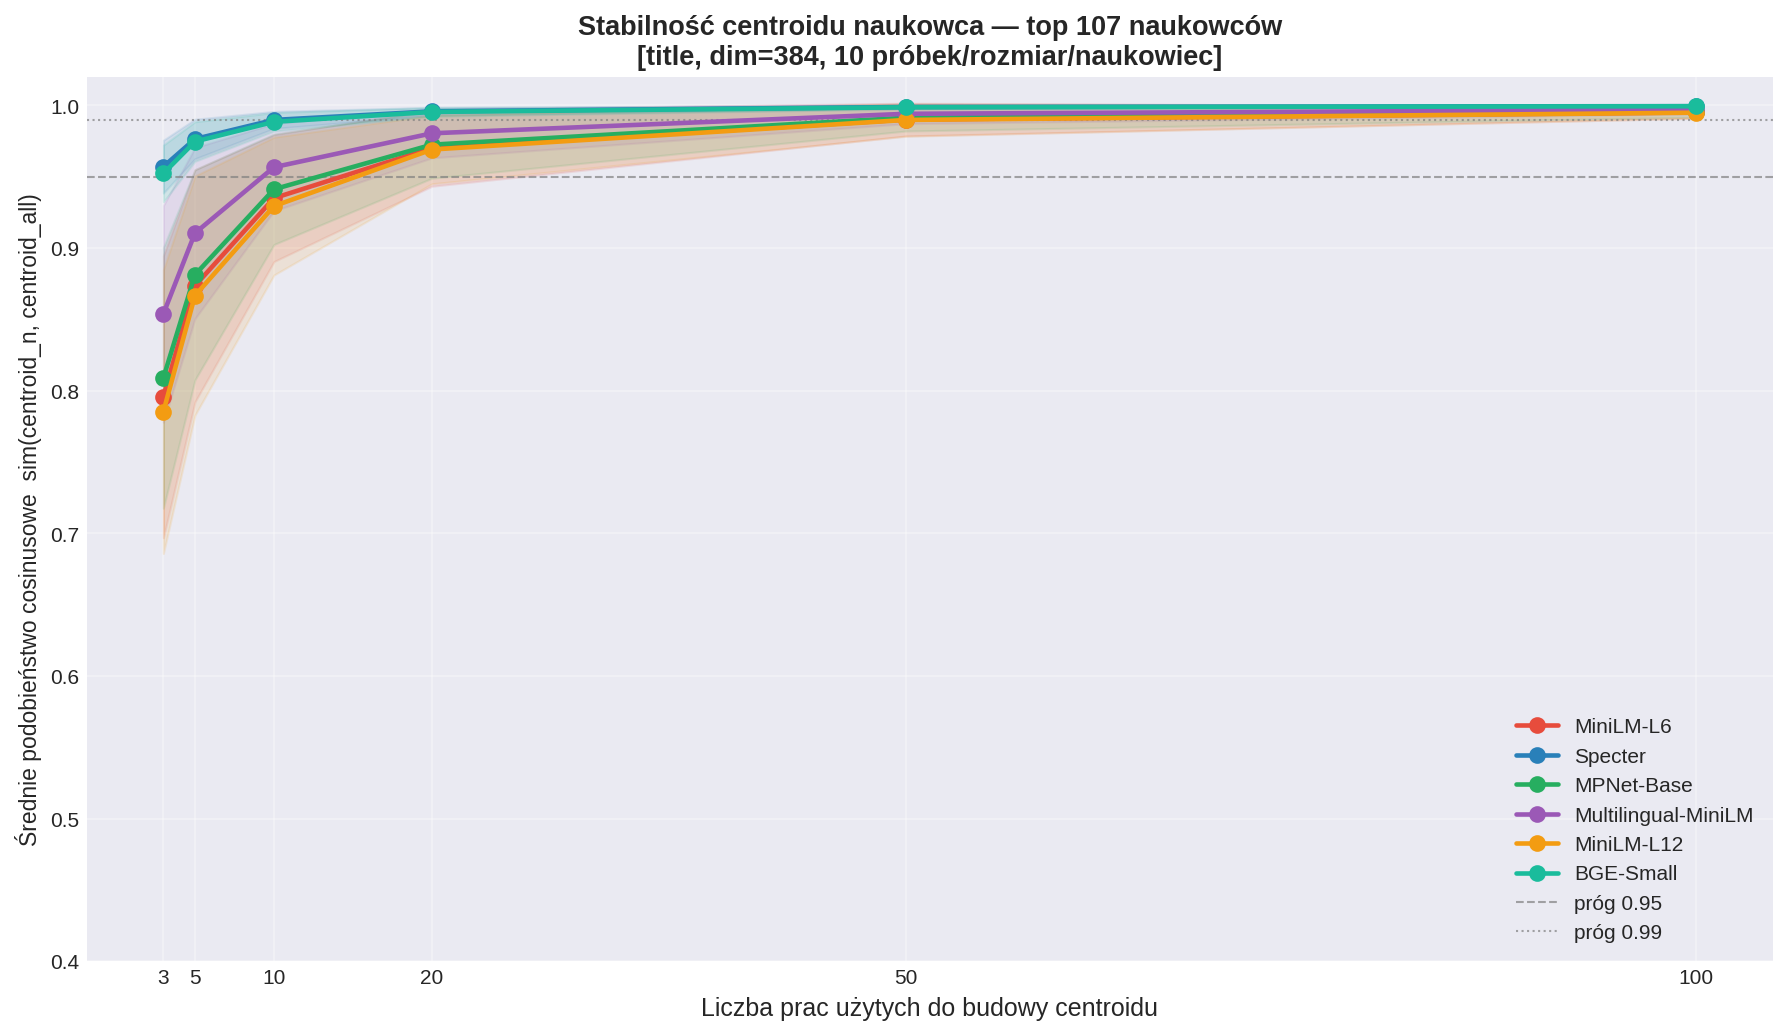
\includegraphics[width=\textwidth]{pubs_num_stability/stability_top_scientists.png}
    \caption{Średnie podobieństwo cosinusowe centroidu próbki do centroidu pełnego
    w~zależności od~liczby prac, uśrednione po~107~naukowcach UAM.
    Każda linia odpowiada innemu modelowi; pasmo ±1~odchylenie standardowe
    ilustruje zmienność między naukowcami.
    Przerywana linia pozioma~-- próg 0{,}95; kropkowana~-- próg 0{,}99.}
    \label{fig:stability_top}
\end{figure}

\begin{table}[H]
\centering
\caption{Średnie podobieństwo cosinusowe $\mathrm{sim}(\mathbf{c}_k,\mathbf{c}_\text{all})$
uśrednione po~naukowcach (eksperyment zbiorczy, 10~losowych podzbiorów/rozmiar/naukowiec).
Kolumna ,,Licz.\ nauk.''\ podaje liczbę naukowców uwzględnionych przy danym~$k$
(naukowcy z~dorobkiem $< k$ są pomijani).}
\label{tab:top_scientists}
\begin{tabular}{r|c|cc|cccc}
\toprule
\textbf{$k$} & \textbf{Licz.} &
\textbf{Specter} & \textbf{BGE-Small} &
\textbf{Multilin.-} & \textbf{MPNet-} & \textbf{MiniLM-} & \textbf{MiniLM-} \\
& \textbf{nauk.} & & & \textbf{MiniLM} & \textbf{Base} & \textbf{L6} & \textbf{L12} \\
\midrule
  3  & 107 & 0{,}9571 & 0{,}9523 & 0{,}8539 & 0{,}8090 & 0{,}7958 & 0{,}7854 \\
  5  & 106 & 0{,}9765 & 0{,}9747 & 0{,}9105 & 0{,}8813 & 0{,}8736 & 0{,}8667 \\
 10  &  88 & 0{,}9898 & 0{,}9885 & 0{,}9567 & 0{,}9412 & 0{,}9350 & 0{,}9294 \\
 20  &  55 & 0{,}9959 & 0{,}9954 & 0{,}9805 & 0{,}9725 & 0{,}9701 & 0{,}9691 \\
 50  &  20 & 0{,}9989 & 0{,}9987 & 0{,}9941 & 0{,}9914 & 0{,}9901 & 0{,}9898 \\
100  &   6 & 0{,}9995 & 0{,}9994 & 0{,}9970 & 0{,}9955 & 0{,}9951 & 0{,}9949 \\
\bottomrule
\end{tabular}
\end{table}

% ----------------------------------------------------------
\subsection{Dyskusja}
% ----------------------------------------------------------

\subsubsection{Dwie klasy modeli}

Wyniki ujawniają wyraźny podział sześciu modeli na~dwie klasy:

\paragraph{Klasa~I -- modele stabilne: Specter i~BGE-Small.}
Oba modele osiągają $\mathrm{sim} > 0{,}95$ już przy~$k = 5$~pracach
(agregat po~107~naukowcach: Specter~$0{,}976$, BGE-Small~$0{,}975$).
Przy $k = 10$ przekraczają próg~$0{,}98$.
Rozrzut odchylenia standardowego w~Exp3 jest wyraźnie mniejszy niż
dla modeli ogólnych, co~świadczy o~jednorodnym zachowaniu
niezależnie od~tego, którego naukowca reprezentujemy.

\paragraph{Klasa~II -- modele wrażliwe: MiniLM-L6, MiniLM-L12, MPNet-Base, Multilingual-MiniLM.}
Przy zaledwie 3~pracach modele te~osiągają jedynie
$0{,}53$--$0{,}63$ (Górecki) lub $0{,}79$--$0{,}85$ (agregat).
Wzrost podobieństwa jest jednak szybki -- przy~$k = 50$
wszystkie cztery modele przekraczają~$0{,}99$ w~eksperymencie zbiorczym,
a~przy~$k = 100$ zbiegają do~wartości porównywalnych z~klasą~I.

\subsubsection{Przyczyny różnic między modelami}

\textbf{Specter} został wytrenowany na~artykułach naukowych
z~sygnałem cytowań (podobne prace cytują się nawzajem)~\cite{specter2020}.
Taka procedura uczenia faworyzuje reprezentacje skupione tematycznie:
prace jednego naukowca lądują w~relatywnie wąskim obszarze przestrzeni,
dlatego centroid stabilizuje się szybko nawet przy małej próbce.

\textbf{BGE-Small} to~model wytrenowany metodą uczenia kontrastywnego
z~trudnymi negatywami (hard negative mining)~\cite{bge2023},
co~sprawia, że~embeddingi są zwarte i~zorientowane tematycznie.
Model ten generuje bardzo skupione reprezentacje dokumentów
z~tej samej dziedziny -- stąd jego wysoka stabilność.

Modele ogólne (MiniLM, MPNet) są optymalizowane na~szerokich
zbiorach zdań z~różnych domen.
Reprezentują one bardziej ,,płaską'' przestrzeń, w~której prace
z~tego samego naukowca mogą być rozrzucone szerzej --
szczególnie gdy naukowiec publikuje w~kilku różnych dziedzinach.
Ilustruje to~przypadek prof.~Góreckiego, którego prace dotyczą
zarówno statystyki funkcjonalnej, jak i~klasyfikacji szeregów
czasowych i~chemometrii żywności.

\subsubsection{Różnica między eksperymentem pilotażowym a~zbiorczym}

Wartości podobieństwa w~Exp3 (agregat) są systematycznie wyższe
niż w~Exp2 dla samego Góreckiego
(np.\ MiniLM-L6, $k=3$: $0{,}530$ vs.\ $0{,}796$).
Wynikają z~tego dwa wnioski.
Po~pierwsze, Górecki ma wyjątkowo szeroki interdyscyplinarny profil,
co~czyni go~trudniejszym przypadkiem niż przeciętny naukowiec.
Po~drugie, przy uśrednianiu po~107~naukowcach część badaczy ma
bardzo skoncentrowane profile (np.\ wąskie specjalności),
co~podnosi średnią.
Oba fakty oznaczają, że~podane progi należy traktować jako
\textbf{oszacowania konserwatywne}: dla typowego naukowca
z~jednorodnym profilem stabilizacja nastąpi szybciej.

\subsubsection{Praktyczne zalecenia dla systemu rekomendacji}

Na~podstawie obu eksperymentów formułujemy następujące wnioski praktyczne:

\begin{itemize}
    \item \textbf{Specter i~BGE-Small} zapewniają stabilny profil już
    przy~\textbf{$k \approx 10$ pracach} ($\mathrm{sim} > 0{,}98$).
    Modele te są zalecanym wyborem, gdy baza danych zawiera naukowców
    z~małym dorobkiem.

    \item \textbf{Modele ogólne} wymagają~\textbf{$k \approx 30$--$50$ prac}
    dla uzyskania $\mathrm{sim} > 0{,}95$.
    Są dobrym wyborem dla naukowców z~bogatym dorobkiem,
    ale~profil naukowców z~mniej niż 20~pracami może być niestabilny.

    \item Dla naukowców z~\textbf{ponad 50~pracami} różnice między modelami
    stają się znikome (wszystkie przekraczają $\mathrm{sim} > 0{,}99$).

    \item Wynik ten sugeruje, że~\textbf{liczba prac jest osobnym wymiarem
    jakości profilu}, niezależnym od~wyboru modelu.
    System rekomendacji powinien informować użytkownika,
    ile prac danego naukowca zostało uwzględnionych w~jego profilu,
    a~ewentualnie przypisywać niższy ,,współczynnik zaufania''
    profilom opartym na~małej liczbie publikacji.
\end{itemize}

% ----------------------------------------------------------
\subsection{Podsumowanie}
% ----------------------------------------------------------

Przeprowadzone eksperymenty wykazały, że~stabilność centroidu profilu naukowca
silnie zależy od~wyboru modelu embeddingowego.
Modele Specter i~BGE-Small -- wytrenowane odpowiednio na~literaturze naukowej
i~za pomocą uczenia kontrastywnego -- tworzą kompaktowe, tematycznie skupione
reprezentacje, dzięki czemu centroid stabilizuje się przy zaledwie 10~pracach.
Modele ogólnego przeznaczenia osiągają porównywalną stabilność dopiero
przy~$\sim$50~pracach.
Wyniki te mają bezpośrednie przełożenie na~decyzję o~wyborze modelu
w~systemie rekomendacji dla środowisk akademickich,
gdzie część naukowców -- zwłaszcza doktoranci i~asystenci --
dysponuje stosunkowo skromnym dorobkiem.

% ============================================================
%  BIBLIOGRAFIA (jeśli używasz bibtex, dodaj do swojego .bib):
% ============================================================
%
%  @inproceedings{specter2020,
%    title   = {{SPECTER}: Document-level Representation Learning
%               using Citation-informed Transformers},
%    author  = {Cohan, Arman and Feldman, Sergey and Beltagy, Iz
%               and Downey, Doug and Weld, Daniel S.},
%    booktitle = {ACL},
%    year    = {2020}
%  }
%
%  @article{bge2023,
%    title   = {{C-Pack}: Packaged Resources To Advance General
%               Chinese Embedding},
%    author  = {Zhang, Peitian and others},
%    journal = {arXiv:2309.07597},
%    year    = {2023}
%  }
%
%  @article{johnson1984extensions,
%    title   = {Extensions of {Lipschitz} mappings into a {Hilbert} space},
%    author  = {Johnson, William B. and Lindenstrauss, Joram},
%    journal = {Contemporary Mathematics},
%    volume  = {26},
%    pages   = {189--206},
%    year    = {1984}
%  }
